\documentclass[11pt]{article}
\usepackage{graphicx} % Required for inserting images
\usepackage{amsmath}
\usepackage{yhmath}
\usepackage{amsthm}
\usepackage{comment}
\usepackage{amssymb,geometry,parskip}
\usepackage[dvipsnames]{xcolor}
\usepackage{todonotes}
\usepackage{mathtools}
\usepackage{pgfplots}
\geometry{tmargin=1in, bmargin=1in, lmargin=1in, rmargin = 1in}
\newcommand{\gonzalo}[1]{{\color{blue} [GMK: {#1}]}}
\usepackage{amsthm}
\newtheorem{theorem}{Theorem}
\newtheorem{claim}{Claim}
\usepackage{tikz}
\usetikzlibrary{matrix}
\usepackage{bbm}
\usepackage{threeparttable}
\usepackage{ragged2e}
\usepackage{float}
\usepackage{physics}

\DeclareMathOperator*{\argmin}{arg\,min}
\DeclareMathOperator*{\argmax}{arg\,max}
\newcommand{\indep}{\perp \!\!\! \perp}

\newcommand{\conv}{\xrightarrow{\;\;\;}}

\newcommand{\convp}{\xrightarrow{{\scriptscriptstyle \mathrm{\;p\;}}}}

\newcommand{\convas}{\xrightarrow{{\scriptscriptstyle \mathrm{a.s.}}}}

\newcommand{\convms}{\xrightarrow{{\scriptscriptstyle \mathrm{m.s.}}}}

\newcommand{\convd}{\xrightarrow{{\scriptscriptstyle \mathrm{\;d\;}}}}

\newcommand{\PP}{\mathbb{P}}

\newcommand{\EE}{\mathbb{E}}
\newcommand{\VV}{\mathbb{V}}

\newcommand{\R}{\mathbb{R}}

\newcommand{\defeq}{\vcentcolon=}

\author{Vaidehi Parameswaran}
\date{\today}

\title{ECON 450-1 Problem Set 4}
\maketitle

\begin{document}

\section*{Question 1}

I plot histograms of prices, profits, and consumer surplus for both simulations, using true parameter values. 

\subsection*{3 Products, 100 Markets}
\begin{figure}[H]
\centering
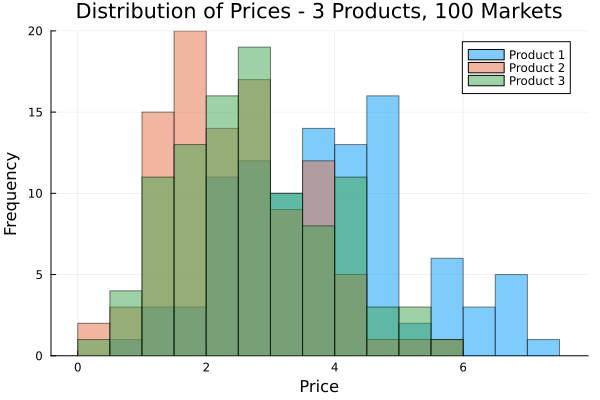
\includegraphics[width=0.8\textwidth]{outputs/prices_3prods_100mkts.png}
\end{figure}

\begin{figure}[H]
\centering
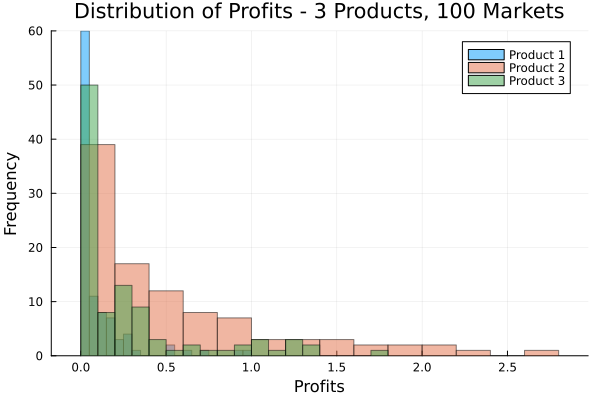
\includegraphics[width=0.8\textwidth]{outputs/profits_3prods_100mkts.png}
\end{figure}

\begin{figure}[H]
\centering
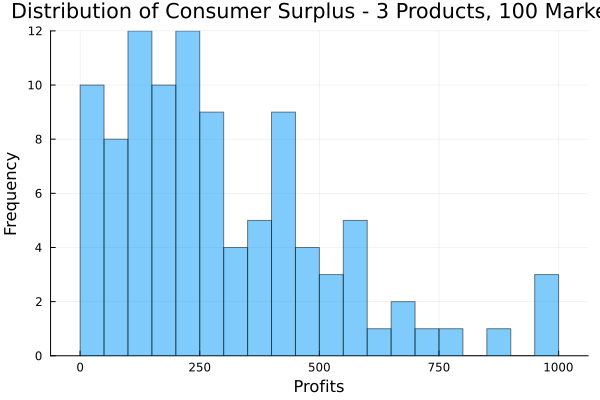
\includegraphics[width=0.8\textwidth]{outputs/cs_3prods_100mkts.png}
\end{figure}
        
\subsection*{5 Products, 100 Markets}

\begin{figure}[H]
\centering
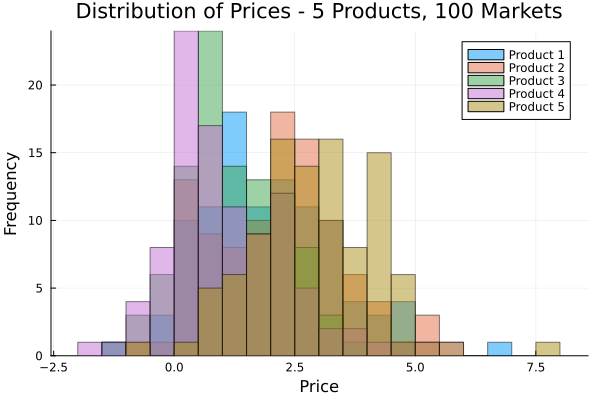
\includegraphics[width=0.8\textwidth]{outputs/prices_5prods_100mkts.png}
\end{figure}

\begin{figure}[H]
\centering
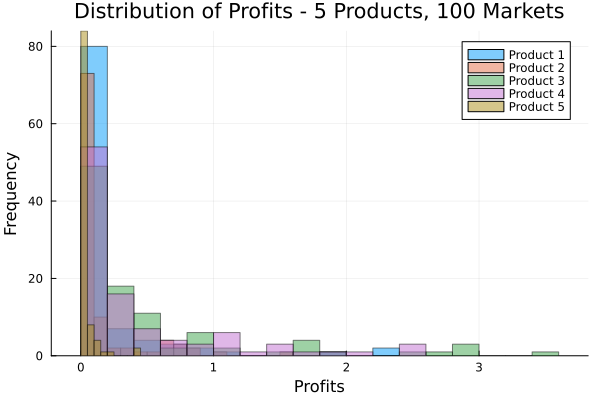
\includegraphics[width=0.8\textwidth]{outputs/profits_5prods_100mkts.png}
\end{figure}

\begin{figure}[H]
\centering
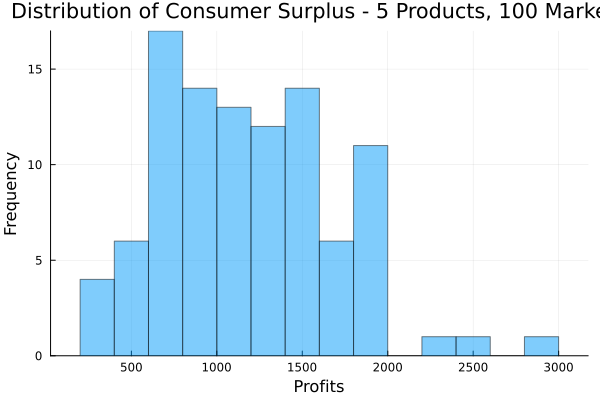
\includegraphics[width=0.8\textwidth]{outputs/cs_5prods_100mkts.png}
\end{figure}

\section*{Question 2}

\subsection*{(2.1)}

\subsubsection*{(a)}
Refer to jupyter notebook for code and results. 

\subsubsection*{(b)}
The first moment condition is part of the BLP instrument set. 
This satisfies relevance because exogenous characteristics of the product will affect prices.
It may or may not satisify the exclusion restriction, based on whether firms can choose these product characteristics

Prices are definitely endogenous, so the exclusion restriction is violated, so the second moment condition may not be valid.

The third moment condition seems to be related to Hausman instruments. 
It satisfies relevance because a change in prices in other markets could signal a change in producer's costs that will affect price in the market of interest.
It may not satisfy exclusion in demand shocks in different markets are correlated.

\subsubsection*{(c)}
Yes, we can use both if we believe that the Hasuman instruments are valid.

\subsection*{(2.2)}

\subsubsection*{(a)}
The BLP moment condition is given by
\begin{align*}
    \EE[\xi_{jm} | Z_{jm}] = 0, Z = \{ X_{jm}, \sum_{i \neq j} x_{2im}, \sum_{i \neq j} x_{3im} \}
\end{align*}

\subsubsection*{(b), (c), (d)}
Refer to code or notebook for this. 
The objective function is fairly simple, and the gradient is also easy.
I was able to use auto differentiation in julia to get the Jacobian for the constraints. 



\subsubsection*{(e)}

I estimate $\theta$. 
I find that the estimates are not too stable across starting values. 
$\beta$ seems to be the most unstable, $\alpha$ and $\sigma$ seem alright. 
Some starting values lead to failure of convergence. I'm not sure why this happening. 
I suspect maybe I need to put soe restrictions on the random generation process of initial values. 
But when it does converge, the estimates are sooo close to the truth, it's a little surprising. 


\subsubsection*{(f)}
Refer to notebook. 

\subsubsection*{(g)}

Repeating estimation for 3 products, 10 markets. 
The estimates are worse, relative to the case with 100 markets, which is expected I suppose.
Faster though!

\subsection*{(2.3)}

I take this question to mean that we can include price in the instrument set and rerun BLP. 
Honestly it doesn't make it that much worse, even though we know prices are endogenous here.
But estimates are a little further from the truth. 
I expected them to be much worse. 
I still have failure of convergence for some starting values. 
I don't have time to explore this further. 

\section*{Question 3}

\subsection*{(3.1)}

\subsubsection*{(a)}

The moment condition is given by
\begin{align*}
    \EE[\xi_{jm} | Z_{jm}] = 0, Z = \{ X_{jm}, \sum_{i \neq j} x_{2im}, \sum_{i \neq j} x_{3im}, W_j\}
\end{align*}

\subsubsection*{(b)}
Refer to code or notebook for this.

\subsubsection*{(c)}
For $M = 10$, the estimates look really bad and far from the true values. 

\subsubsection*{(d)}


\subsection*{(3.2)}

I have to give up here...

\end{document}